\documentclass[oneside, final]{scrartcl}
\usepackage{url}
%\raggedright
\parindent 0in
\parskip 10pt plus 1pt minus 10pt

%\pagestyle{empty}

% MARGINS:

\oddsidemargin  0pt % was 38
\evensidemargin 0pt % was 38
\marginparwidth 0pt % was 68

\topmargin  15pt   % was 27
\headheight  0pt   % was 12
\headsep     0pt   % was 25
%\footheight  0pt   % was 12
\footskip   30pt   % was 30

\textwidth  466pt    % was 390pt
\textheight 650pt  % was 536.5

%\renewcommand{\ul}[1]{\underline{\vphantom{y}#1}}
\makeatletter

\def\entrieslabel#1{\hspace\labelsep#1:}
\newenvironment{entries}
  {\list{}{\labelwidth\z@
      \leftmargin 40pt
      \rightmargin 0pt
      \listparindent -15pt
      \itemindent-\leftmargin
      \let\makelabel\entrieslabel}}{\endlist}
\newcommand{\entry}[1]{\item[\sc #1]\mbox{}}
\newcommand{\nullentry}[1]{\item\mbox{}}

\makeatother

\newlength{\hdlm}
\newlength{\oldlm}

\newcommand{\hditem}[1]{\protect\item[#1\hfill]}

\newenvironment{hangingdesc}[1]{\begin{list}{}%
{\setlength{\oldlm}{\leftmargin}
\settowidth{\leftmargin}{#1}%
%\addtolength{\hdlm}{\leftmargin}%
%\setlength{\leftmargin}{\hdlm}%
\settowidth{\labelwidth}{{\bf #1}\hspace*{0.1in}}}}%
{\setlength{\leftmargin}{\oldlm}\end{list}}



\usepackage{soul}
\usepackage{scrpage2}
\usepackage{titlesec}
\usepackage{palatino}
\usepackage{textcomp}
\usepackage{multicol}

\usepackage{hyperref}
\hypersetup{
    colorlinks=true,
    linkcolor=blue,
    filecolor=magenta,      
    urlcolor=black,
}
 
\urlstyle{same}
\usepackage{amsmath,amsfonts,amsthm} 
\usepackage[pdftex]{graphicx} 
\usepackage[svgnames]{xcolor} 
\usepackage{url} 
\usepackage{wrapfig}

\frenchspacing 
\pagestyle{empty}

\usepackage{sectsty} 
    \sectionfont{% 
        \usefont{OT1}{ph}{b}{n}% 
        \sectionrule{0pt}{0pt}{-5pt}{1.5pt} }
    \subsectionfont{% 
        \usefont{OT1}{ph}{b}{n}% 
        \sectionrule{0pt}{0pt}{-5pt}{0pt} }%\allsectionsfont{\sffamily\mdseries\upshape}


\usepackage[text={6in,9in},centering]{geometry}

\titleformat{\section}{\large\scshape\raggedright}{}{0em}{}[\titlerule]

\begin{document}
%\begin{center}

\begin{center}
\textsc{\huge{\so{William L. Harrison, Ph.D}}}
\\[2ex]
1238 Sunset Drive, Columbia Missouri 65201
\\
\href{https://harrisonwl.github.io}{https://harrisonwl.github.io}
\\
harrisonwl@missouri.edu
\end{center}

\section*{Education}

%\begin{entries}
%\nullentry{}
\begin{hangingdesc}{}
\hditem{May 2001.}
Ph.D., Computer Science, University of Illinois, Urbana, IL. \\
	    Dissertation: ``Modular Compilers and Their Correctness Proofs."
	\\Committee Chairman:  Samuel Kamin

\hditem{June 1992.}
    M.S., Computer Science, University of California, Davis, CA.\\ Thesis: ``Mechanizing the Axiomatic Semantics for a Programming Language with Asynchronous Send and Receive in HOL.''


\hditem{June 1986.}
    B.A., Mathematics,
	     University of California, Berkeley, CA.


\end{hangingdesc}
%\end{entries}

%%%%%%%%%%%%%%%%%%%%%%%%%%%%%%%%%%%%%
%%%%%%%%%%%%%%%%%%%%%%%%%%%%%%%%%%%%%
%%%%%%%%%%%%%%%%%%%%%%%%%%%%%%%%%%%%%
%%%%%%%%%%%%%%%%%%%%%%%%%%%%%%%%%%%%%
%%%%%%%%%%%%%%%%%%%%%%%%%%%%%%%%%%%%%
\section*{Academic Appointments \& Professional Experience}
\begin{hangingdesc}{}

\hditem{August 2013--July 2014.} {\bf Visiting Scientist}, National Security Agency.

\hditem{April 2011--present.} {\bf Director}, The Center for High Assurance Computing at the University of Missouri.

\hditem{Sept. 2003--present.} {\bf Associate Professor}, Department of Computer
Science,
University of Missouri at Columbia,
Columbia, Missouri. Started as assistant professor; earned promotion and tenure 5/26/2009. 

\hditem{Sept. 2010--present.} {\bf Research Associate}, Pro-telligent, Inc. 
Arlington, Virginia.

\hditem{June 2000--August 2003.} {\bf Senior Research Associate \& Adjunct Professor}, Computer
Science Department,
OGI School of Science \& Engineering,
Oregon Health \& Sciences University.

\hditem{Sept. 2000--Dec. 2000.} {\bf Senior Compiler Engineer (consultant)}, Reservoir
Laboratories, Portland, Oregon.

\hditem{August 1999--May 2000.}
    {\bf Visiting Lecturer}, Department of Computer Science,
	Indiana University, Bloomington, IN 47401.
\hditem{Spring 1999.}
	{\bf Visiting Lecturer}, Department of Computer Science,
	  University of Illinois at Urbana-Champaign, Urbana, IL.

\end{hangingdesc}



%%%%%%%%%%%%%%%%%%%%%%%%%%%
%%%%%%%%%%%%%%%%%%%%%%%%%%%
%%%%%%%%%%%%%%%%%%%%%%%%%%%
%%%%%%%%%%%%%%%%%%%%%%%%%%%
%%%%%%%%%%%%%%%%%%%%%%%%%%%
\section*{Research Interests}

\begin{hangingdesc}{}

\hditem{}
Computer security and
language-based methods in security; Trustworthy computing; Formal methods (particularly with respect to
hardware/software codesign);  Programming language
design and implementation.

\end{hangingdesc}


%%%%%%%%%%%%%%%%%%%%%%%%%%%
%%%%%%%%%%%%%%%%%%%%%%%%%%%
%%%%%%%%%%%%%%%%%%%%%%%%%%%
%%%%%%%%%%%%%%%%%%%%%%%%%%%
%%%%%%%%%%%%%%%%%%%%%%%%%%%%
\section*{Personal Information}

\begin{hangingdesc}{}
\hditem{} I am a US citizen.
\vspace{-1ex}
%\hditem{} I have a Top Secret/SCI security clearance.
%\vspace{-1ex}
\hditem{} I am married to Amber Bradshaw, who is a ceramic artist.
\vspace{-1ex}

\hditem{} We have two children: Tegan and Caden (twins, 8 years old). 
\vspace{-1ex}

\end{hangingdesc}


%%%%%%%%%%%%%%%%%%%%%%%%%%%%%%%%%
%%%%%%%%%%%%%%%%%%%%%%%%%%%%%%%%%
%%%%%%%%%%%%%%%%%%%%%%%%%%%%%%%%%
%%%%%%%%%%%%%%%%%%%%%%%%%%%%%%%%%
%%%%%%%%%%%%%%%%%%%%%%%%%%%%%%%%%
\section*{Funding History}

\subsection*{\it Active Grants and Contracts}

\begin{hangingdesc}{}
\hditem{$1.$}
{\bf Agency:} US Naval Research Laboratory.
\\
{\bf Title:} Mechanizing the Metatheory of the ReWire Language with Applications.
\\
{\bf Amount:} \$720,000.
\\
{\bf Period:}   May 2016  --  August 2019.
\\
{\bf Role:}    Sole  Principal investigator.
\end{hangingdesc}


\subsection*{\it Completed Grants and Contracts}
\begin{hangingdesc}{}
\hditem{$2.$}
{\bf Agency:} US Naval Research Laboratory.
\\
{\bf Title:} Type-Based Analysis of Security Flows in ReWire Circuit Specifications.
\\
{\bf Amount:} \$99,999.
\\
{\bf Period:}   October 2014  --  October 2015.
\\
{\bf Role:}     Sole Principal investigator.
\end{hangingdesc}

\begin{hangingdesc}{}
\hditem{$3.$}  {\bf Agency:} National Security Agency.\\
               {\bf Title:} Inter-agency Personnel Agreement.\\
               {\bf Amount:} \$144,190.00 \\
               {\bf Period:} August 2013 -- August 2014.

\hditem{$4.$}
{\bf Agency:} Department of Defense, Federal Voting Assistance Program (FVAP).
\\
{\bf Title:} Secure Ballot Delivery to UOCAVA Voters (Uniformed, Overseas, Citizens Absentee Voters). 
\\
{\bf Amount:} \$550,000.
\\
{\bf Period:} May 1, 2012 -- April 30, 2015.
\\
{\bf Role:} Collaborative research with Dr. Dale Musser of MU's Information Technology Program and Dr. Keith Politte of MU's Reynolds School of Journalism. 

\hditem{$5.$}
{\bf Agency:} Department of Education.
 ~\\
{\bf Title:} Graduate Assistance in Areas of National Need (GAANN) Fellowships.
\\
{\bf Amount:} \$240,000.
\\
{\bf Period:} September 1, 2011 -- May 15, 2015.
\\
{\bf Role:} Co-Investigator. Two of my Ph.D students (Adam Procter and Christopher Hathhorn) are GAANN fellows. 

\hditem{$6.$}
{\bf Agency:} National Science Foundation.
\\
{\bf Title:} CAREER: Automated Synthesis of High Assurance Security Kernels.
\\
{\bf Amount:} \$450,000.
\\
{\bf Period:}   June 1, 2008  --  May 31, 2013.
\\
{\bf Role:}      Sole Principal Investigator.

\hditem{$7.$}
{\bf Agency:} Office of the Asst. Secretary of Defense for Research and Development (ASD(R\&E)).
\\
{\bf Title:} Understanding Security Flows in the Many Core Era.
\\
{\bf Amount:} \$1,370,000.
\\
{\bf Period:}   January 2012  --  July 2015.
\\
{\bf Role:}      Principal Investigator. Collaborative Research with Dr. David Andrews (University of Arkansas) and Dr. Gerard Allwein (NRL).
\end{hangingdesc}

\begin{hangingdesc}{}
\hditem{$8.$}
{\bf Agency:} US Naval Research Laboratory.
\\
{\bf Title:} MILS Hardware and Its Formal Methods-based Security.
\\
{\bf Amount:} \$810,000.
\\
{\bf Period:}   April 2008  --  April 2011.
\\
{\bf Role:}      Principal Investigator. Collaborative Research with Dr. David Andrews (University of Arkansas) and Dr. Gerard Allwein (NRL).


\hditem{$9.$}
{\bf Agency:} Department of Defense through OHSU/OGI.
\\
{\bf Title:} System Information Assurance II
\\
{\bf Amount:} \$31,703 
\\
{\bf Period:}   July 1, 2004  --  July 31, 2006
\\
{\bf Role:}      Principal Investigator

\hditem{$10.$}
{\bf Agency:} University of Missouri-Columbia Research Council.
\\
{\bf Title:} Big Twelve Faculty Fellowship
\\
{\bf Amount:} \$2,400
\\
{\bf Period:}   June 1, 2006  --  August 31, 2006 
\\
{\bf Role:}      Sole Principal Investigator
\end{hangingdesc}

%%%%%%%%%%%%%%%%%%%%%%%%%%%
%%%%%%%%%%%%%%%%%%%%%%%%%%%
%%%%%%%%%%%%%%%%%%%%%%%%%%%
%%%%%%%%%%%%%%%%%%%%%%%%%%%
%%%%%%%%%%%%%%%%%%%%%%%%%%%
\section*{Publications}

%%%%%%%%%%%%%%%
%%%%%%%%%%%%%%%
%%%%%%%%%%%%%%%
\subsection*{\it{Book Chapters}}

\begin{hangingdesc}{}


\hditem{}
Gerard Allwein and William L. Harrison.
\newblock Distributed Modal Logic.
\newblock {\it J. Michael Dunn on Information Based Logics, Book Chapter, pages 331-362, Springer Verlag, 2016}.

\end{hangingdesc}

%%%%%%%%%%%%%%%
%%%%%%%%%%%%%%%
%%%%%%%%%%%%%%%
\subsection*{\it{Journal Publications}}

\begin{hangingdesc}{}

\hditem{}
Gerard Allwein, William L. Harrison, and Thomas Reynolds.
\newblock Distributed Relation Logic.
\newblock {\it Logic and Logical Philosophy}, volume 26, number 1, March 2017, pages 19-61.


\hditem{}
Adam Procter, William L. Harrison, Ian Graves, Michela Becchi, and Gerard Allwein.
\newblock A Principled Approach to Secure Multi-Core Processor Design with ReWire
\newblock {\it ACM Transactions on Embedded Computing Systems}, volume 16, number 2, Article 33 (January 2017), 25 pages.


\hditem{}
Gerard Allwein, William Harrison and David Andrews.
\newblock Simulation logic.
\newblock {\it Logic and Logical Philosophy, vol. 26, no. 3}, 2014.

\hditem{}
G.~Allwein, Y.~Yang, and W.~L. Harrison.
\newblock Qualitative decision theory via channel theory.
\newblock {\em Logic and Logical Philosophy}, Volume 20, Number 1-2 (2011), pages 81--110.

\hditem{}
W.~L. Harrison and J.~Hook.
\newblock Achieving information flow security through monadic control of
  effects.
\newblock {\em Journal of  Computer Security}, 17:599--653, October 2009.

\hditem{}
X.~Z. Fu, H.~Wang, W.~L. Harrison, and R.~Harrison.
\newblock {RNA} pseudoknot prediction using term rewriting.
\newblock {\em International Journal of Data Mining and Bioinformatics}, 2(1):78-93, February 2008.

\hditem{}
W.~L. Harrison and R.~B. Kieburtz.
\newblock The logic of demand in {H}askell.
\newblock {\em Journal of Functional Programming}, 15(6):837--891, 2005.


\hditem{}
W.~L. Harrison.
\newblock Cheap (but functional) threads.
\newblock 44 pages. Accepted for publication in: {\em Higher-Order Symbolic Computation}. Please see the commentary on this article below.

\end{hangingdesc}

%%%%%%%%%%%%%%%
%%%%%%%%%%%%%%%
%%%%%%%%%%%%%%%
\subsection*{{\it Under Submission}}

\begin{hangingdesc}{}


\hditem{}
Gerard Allwein, William Harrison and Thomas Reynolds.
\newblock Channel Theory and Information Flow.
\newblock {\it Journal of Applied Non-classical Logic}, 2016.


\end{hangingdesc}

%%%%%%%%%%%%%%%
%%%%%%%%%%%%%%%
%%%%%%%%%%%%%%%
\subsection*{{\it Peer-reviewed Conference Publications}}

\begin{hangingdesc}{}

\hditem{} 
Thomas N. Reynolds, Adam Procter, William L. Harrison, and Gerard Allwein.
\newblock A Core Calculus for Secure Hardware: Its Formal Semantics and Proof System.
\newblock {\it Proceedings of the 15th ACM-IEEE International Conference on Formal Methods and Models for System Design (MEMOCODE17)}, 2017 (to appear).


\hditem{}
William L. Harrison, Adam Procter, and Gerard Allwein.
\newblock Model-driven Design \& Synthesis of the SHA-256 Cryptographic Hash Function in ReWire.
\newblock {\it Proceedings of the 27th International Symposium on Rapid System Prototyping (RSP), 2016}.

\hditem{}
William L. Harrison, Adam Procter, Ian Graves, Michela Becchi, and Gerard Allwein. 
\newblock A Programming Model for Reconfigurable Computing Based in Functional Concurrency.
\newblock {\it Proceedings of the 11th International Symposium on Reconfigurable Communication-centric Systems-on-Chip (ReCoSoC 2016)}.

\hditem{}
Ian Graves, Adam Procter, William L. Harrison, and Gerard Allwein.
\newblock Provably Correct Development of reconfigurable hardware designs via equational reasoning.
\newblock {\it Proceedings of the 2015 International Conference on
Field-Programmable Technology (FPT '15)}.

\hditem{}
Adam Procter, William L. Harrison, Ian Graves, Michela Becchi, and Gerard Allwein. 
\newblock Semantics driven hardware design, implementation, and verification with ReWire. 
\newblock {\it ACM SIGPLAN/SIGBED Conf. on Languages, Compilers, Tools and Theory for Embedded Systems (LCTES), 2015.} 

\hditem{}
Ian Graves, Adam Procter, William L. Harrison, Michela Becchi and Gerard Allwein.
\newblock Hardware Synthesis from Functional Embedded Domain-Specific Languages.
\newblock {\it Proceedings of the 2015 11th International Symposium on 
Applied Reconfigurable Computing}.


\hditem{}
Adam Procter, William L. Harrison, Ian Graves, Michela Becchi and Gerard Allwein.
\newblock Semantics-directed Machine Architecture in ReWire.
\newblock {\it Proceedings of the 2013 International Conference on Field Programmable Technology.}

\hditem{}
Robert Harrison and William L. Harrison.
\newblock Quantitative Analysis of Error Injection Covert Channels.
\newblock {\it Proceedings of the International Workshop on Quantitative Aspects in Security Assurance (QASA 2013).}

\hditem{}
   William L. Harrison, Adam Procter and Gerard Allwein.
\newblock The Confinement Problem in the Presence of Faults.
\newblock {\it Proceedings of the 2012 International Conference on Formal Engineering Methods.}
                  
\hditem{}
Chris Hathhorn, Michela Becchi, William L. Harrison and Adam Procter
\newblock Formal Semantics of Heterogeneous CUDA-C: A Modular Approach with Applications.
\newblock {\it Proceedings of the 2012 Systems Software Verification Conference.}

\hditem{}
Gerard Allwein, William L. Harrison and David Andrews.
\newblock Simulation Logic.
\newblock {\it Proceedings of the 2012 Conference on Non-Classical Logics.}

\hditem{}
 Adam Procter, William L. Harrison and Aaron Stump.
 \newblock The Design of a Practical Proof Checker for a Lazy Functional Language.
 \newblock {\it Proceedings of the 2012 Trends in Functional Programming Conference.}

\hditem{}
W.~L. Harrison, B.~Schulz, A.~Procter, A.~Lukefahr, and G.~Allwein.
\newblock Towards semantics-directed system design and synthesis.
\newblock In {\em Proceedings of the 2011 International Conference on
  Engineering Reconfigurable Systems and Algorithms (ERSA11)}, 2011.



\hditem{}
G.~Allwein and W.~L. Harrison.
\newblock A channel theoretic account of separation security.
\newblock In {\em Proceedings of the 2011 International Conference on
  Engineering Reconfigurable Systems and Algorithms (ERSA11)}, 2011.


\hditem{}
G.~Allwein, Y.~Yang, and W.~L. Harrison.
\newblock Decision theory via channel theory.
\newblock In {\em Proceedings of the Logic in Cognitive Science Conference}. The Nicolaus Copernicus
  University Press, 2010.

\hditem{}
G.~Allwein and W.~L. Harrison.
\newblock Partially-ordered modalities.
\newblock In {\em Proceedings of the Advances in Modal Logic (AiML) Conference}, pages 1--21, 2010.

\hditem{}
W.~L. Harrison, A.~Procter, J.~Agron, G.~Kimmel, and G.~Allwein.
\newblock Model-driven engineering from modular monadic semantics:
  Implementation techniques targeting hardware and software.
\newblock In {\em DSL '09: Proc. of the IFIP TC 2 Working Conference on
  Domain-Specific Languages}, pages 20--44, 2009.



\hditem{}
W.~L. Harrison, G.~Allwein, A.~Gill, and A.~Procter.
\newblock Asynchronous exceptions as an effect.
\newblock In {\em Proceedings of the Mathematics of Program Construction
  (MPC08)}, pages 153--176, 2008.



\hditem{}
P.~S. Kariotis, A.~M. Procter, and W.~L. Harrison.
\newblock Making monads first-class with template haskell.
\newblock In {\em Proceedings of the first ACM SIGPLAN Symposium on Haskell},
  Haskell '08, pages 99--110, New York, NY, USA, 2008. ACM.

\hditem{}
W.~L. Harrison.
\newblock The essence of multitasking.
\newblock In {\em 11th International Conference on Algebraic Methodology and
  Software Technology {(AMAST 2006)}}, pages 158--172, July 2006.


\hditem{}
W.~L. Harrison.
\newblock Proof abstraction for imperative languages.
\newblock In {\em Proceedings of the 4th Asian Symposium on Programming
  Languages and Systems (APLAS06)}, pages 97--113, 2006.

\hditem{}
W.~L. Harrison and J.~Hook.
\newblock Achieving information flow security through precise control of
  effects.
\newblock In {\em 18th IEEE Computer Security Foundations Workshop (CSFW05)},
  pages 16--30, Aix-en-Provence, France, June 2005.

\hditem{}
W.~L. Harrison.
\newblock A simple semantics for polymorphic recursion.
\newblock In {\em Proceedings of the 3rd Asian Symposium on Programming
  Languages and Systems (APLAS05)}, pages 37--51, Tsukuba, Japan, November
  2005.

\hditem{}
X.~Z. Fu, H.~Wang, W.~L. Harrison, and R.~Harrison.
\newblock {RNA} pseudoknot prediction using term rewriting.
\newblock In {\em Proceedings of IEEE Fifth Symposium on Bioinformatics and
  Bioengineering (BIBE05)}, pages 169--176, Minneapolis, MN, October 2005.

\hditem{}
W.~L. Harrison and R.~W. Harrison.
\newblock Domain specific languages for cellular interactions.
\newblock In {\em Proceedings of the 26th Annual IEEE International Conference
  on Engineering in Medicine and Biology (EMBC04)}, September 2004.

\hditem{}
W.~L. Harrison, M.~Tullsen, and J.~Hook.
\newblock Domain separation by construction.
\newblock In {\em LICS03 Satellite Workshop on Foundations of Computer Security
  (FCS03)}, June 2003.
\newblock 21 pages.

\hditem{}
W.~L. Harrison, T.~Sheard, and J.~Hook.
\newblock Fine control of demand in {Haskell}.
\newblock In {\em 6th International Conference on the Mathematics of Program
  Construction (MPC02), Dagstuhl, Germany}, volume 2386 of {\em Lecture Notes in Computer Science}, pages 68--93. 2002.



\hditem{}
W.~L. Harrison and R.~Kieburtz.
\newblock Pattern-driven reduction in haskell.
\newblock In {\em 2nd International Workshop on Reduction Strategies in
  Rewriting and Programming (WRS02)}, Copenhagen, Denmark, 2002.


\hditem{}
W.~L.~Harrison and T.~Sheard.
\newblock Dynamically adaptable software with metacomputations in a staged
  language.
\newblock In {\em Proceedings of the Second International Workshop on
  Semantics, Applications, and Implementation of Program Generation (SAIG)},
  volume 2196 of {\em Lecture Notes in Computer Science}, pages 163--182,
  Florence, Italy, 2001. Springer-Verlag.


\hditem{}
W.~L. Harrison and S.~Kamin.
\newblock Metacomputation-based compiler architecture.
\newblock In {\em 5th International Conference on the Mathematics of Program
  Construction, Ponte de Lima, Portugal}, volume 1837 of {\em Lecture Notes in
  Computer Science}, pages 213--229. Springer-Verlag, 2000.


\hditem{}
W.~L. Harrison and S.~N. Kamin.
\newblock Modular compilers based on monad transformers.
\newblock In {\em Proceedings of the 1998 International Conference on Computer
  Languages}, pages 122--131. IEEE Computer Society Press, 1998.


\hditem{}
W.~L. Harrison, K.~Levitt, and M.~Archer.
\newblock An {HOL} mechanization of the axiomatic semantics of a simple
  distributed programming language.
\newblock In {\em Proceedings of the International Workshop on Higher-Order
  Logic Theorem Proving and Its Applications}, pages 347--358, Leuven, Belgium,
  September 1992.

\hditem{}
W.~L. Harrison and K.~Levitt.
\newblock Mechanizing security in {HOL}.
\newblock In {\em Proceedings of the 1991 International Workshop on the {HOL}
  Theorem Proving System and its Applications}, pages 63--66, Davis,
  California, 1991. IEEE Computer Society Press.

\end{hangingdesc}

%%%%%%%%%%%%%%%
%%%%%%%%%%%%%%%
%%%%%%%%%%%%%%%
\subsection*{{\it Dissertation and Master's Thesis}}

\begin{hangingdesc}{}

\hditem{}
W.~L. Harrison.
\newblock {\em Modular Compilers and Their Correctness Proofs}.
\newblock PhD thesis, University of Illinois at Urbana-Champaign, 2001.

\hditem{}
W.~L. Harrison.
\newblock \emph{Mechanizing the axiomatic semantics for a programming language with
  asynchronous send and receive in {HOL}.}
\newblock Master's thesis, University of California, Davis, 1992.


\end{hangingdesc}

%%%%%%%%%%%%%%%
%%%%%%%%%%%%%%%
%%%%%%%%%%%%%%%
\subsection*{{\it Technical Reports}}



\begin{hangingdesc}{}

\hditem{}
Gerard Allwein and William L. Harrison.
\newblock {Distributed Logics}.
\newblock Technical Report NRL/MR/5540-14-9565, US Naval Research Laboratory, 2014. 

\hditem{}
W.~L. Harrison.
\newblock {Mechanizing the Axiomatic Semantics for a Programming Language with
  Asynchronous Send and Receive in HOL}.
\newblock Technical Report CSE-92-20, University of California at Davis, 1992.


\hditem{}
W.~Harrison, K.~Levitt, and M.~Archer.
\newblock {Towards a Verified Code Basis for a Secure Distributed Operating
  System}.
\newblock Technical Report CSE-92-19, University of California at Davis, 1992.

\end{hangingdesc}

%%%%%%%%%
%%%%%%%%%
%%%%%%%%%
\subsection*{Comment on ``Cheap (But Functional) Threads''}

I submitted the article ``\emph{Cheap (But Functional) Threads}'' (CBFT) to the prestigious journal Higher-Order Symbolic Computation (HOSC) in 2008, and it was fully peer-reviewed and then accepted for publication by the HOSC editor-in-chief, Oliver Danvy in email in 2009:
\begin{center}
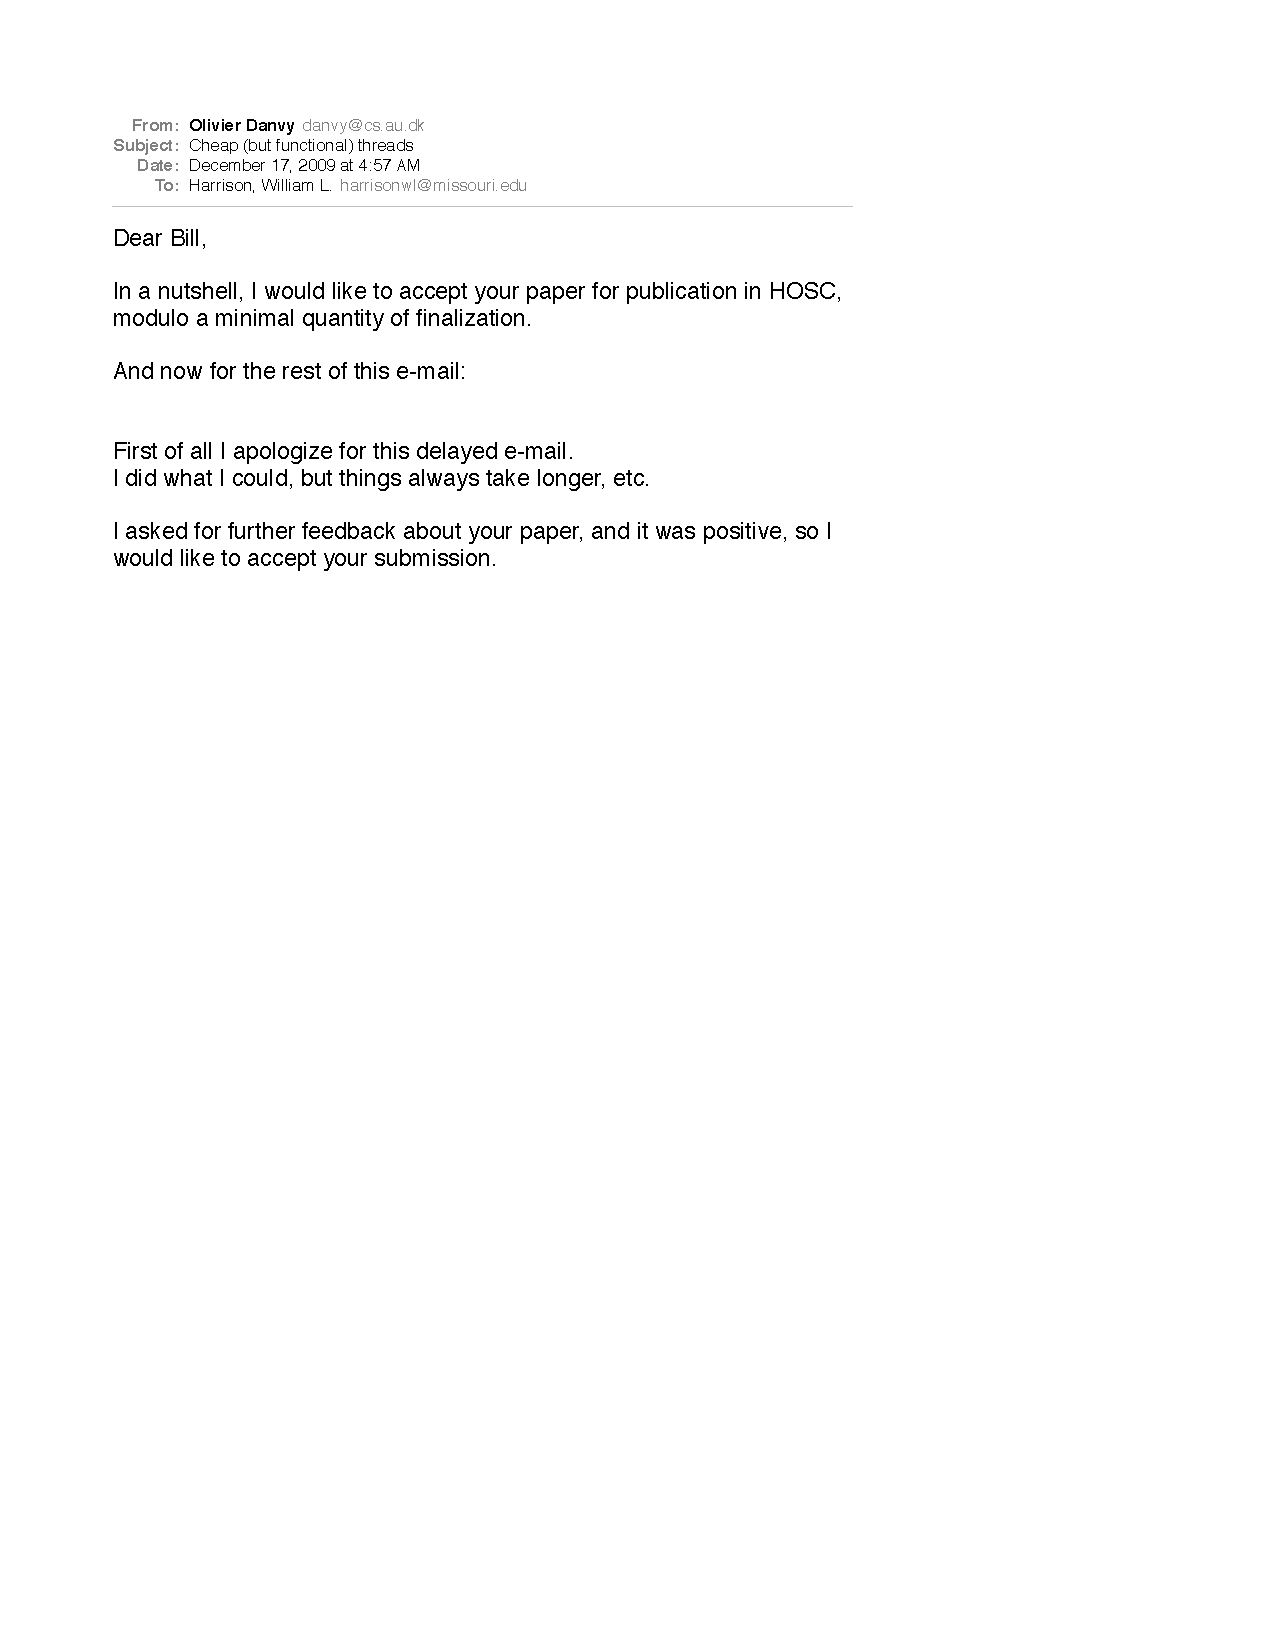
\includegraphics[scale=0.7]{cheapthreads/OlivierAccepts.pdf}
\end{center}
I have removed the remainder of the email as it involves only specific editing details, etc.

CBFT is a journal version of an earlier conference publication ``\emph{The Essence of Multitasking}'' (AMAST 2006) and a pre-print version of the article has been present on my website for ten years or so. A number of researchers have made use of and cited CBFT; here's a list of recent citations:
\begin{itemize}
\item
Pablo Buiras, Amit Levy, Deian Stefan, Alejandro Russo, and David Mazi\'{e}res.
\newblock A library for removing cache-based attacks in concurrent information
  flow systems.
\newblock In Mart\'{i}�n Abadi and Alberto Lluch~Lafuente, editors, {\em
  Trustworthy Global Computing}, volume 8358 of {\em Lecture Notes in Computer
  Science}, pages 199--216. Springer International Publishing, 2014.

\item
Simon Marlow, Louis Brandy, Jonathan Coens, and Jon Purdy.
\newblock There is no fork: An abstraction for efficient, concurrent, and
  concise data access.
\newblock In {\em Proceedings of the 19th ACM SIGPLAN International Conference
  on Functional Programming}, ICFP '14, pages 325--337, New York, NY, USA,
  2014. ACM.

\item
Hannes Mehnert and David~Kaloper Mer\v{s}inak.
\newblock Transport layer security purely in ocaml.
\newblock In {\em OCaml Developers and Users Workshop}, 2014.

\item
Jaakko Pallari.
\newblock Multithread concurrency in a single thread environment.
\newblock Master's thesis, University of Jyv\"{a}skyl\"{a}, 2015.

\item
Maciej Pir{\'{o}}g and Jeremy Gibbons.
\newblock Tracing monadic computations and representing effects.
\newblock In {\em Proceedings Fourth Workshop on Mathematically Structured
  Functional Programming, {MSFP} 2012, Tallinn, Estonia, 25 March 2012.}, pages
  90--111, 2012.

\item
Wouter Swierstra.
\newblock {\em A functional specification of effects}.
\newblock PhD thesis, University of Nottingham, July 2009.

\end{itemize}

CBFT has not yet appeared in print, despite having been accepted for publication at HOSC since late 2009. It is not clear, at this point, whether HOSC is still in operation. I have attempted to contact Olivier Danvy many, many times over the past several years to clarify the situation with HOSC and CBFT, but he has been unresponsive.


%The rest of that paragraph was too personal and giving them information they do not need and seems to indicate you and this fellow do not get along. Shortening it leaves it as ?you do not know what their issue is?. Also, do not use contractions like ?isn?t? in technical writing. 
%
%I would change the following paragraph to

CBFT has been extensively peer-reviewed, been accepted for publication at a prestigious journal, and has been, and continues to be, cited and downloaded from my web site by researchers in the programming languages community. 

%%%%%

%CBFT has not yet appeared in print, despite having been accepted for publication at HOSC since late 2009. It isn't clear, at this point, whether HOSC is still in operation. I have attempted to contact Olivier Danvy many, many times over the past several years to clarify the situation with HOSC and CBFT, but he has been unresponsive. Olivier is an extremely brilliant and prominent member of the programming languages community. He and I have always been on friendly terms---he, in fact, was extremely supportive of my tenure case at MU and wrote a fantastic reference letter for me. But, to be blunt, he has become increasingly erratic and eccentric over the past ten years.

%The bottom line is that CBFT has been extensively peer-reviewed, been accepted for publication at a prestigious journal, and has been, and continues to be, cited by researchers in the programming languages community, but it has not yet appeared in print.

%%%%%%%%%%%%%%%%%%%%%%%%%%%%%%%%%
%%%%%%%%%%%%%%%%%%%%%%%%%%%%%%%%%
%%%%%%%%%%%%%%%%%%%%%%%%%%%%%%%%%
%%%%%%%%%%%%%%%%%%%%%%%%%%%%%%%%%
%%%%%%%%%%%%%%%%%%%%%%%%%%%%%%%%%
\section*{Selected Honors, Memberships, and Service}

\begin{hangingdesc}{}
\hditem{$\bullet$} Selected for Intel Corporation's 2017 Hardware Accelerator Research Program.

\hditem{$\bullet$} Program Chair for 
Seventh Workshop on Design, Modeling and Evaluation of Cyber Physical Systems (CyPhy'17).

\hditem{$\bullet$} Organized special session entitled \emph{The Confluence of Secure Hardware and Programming Languages} for the International Conference on 
Engineering of Reconfigurable Systems and Algorithms (ERSA 11).

\hditem{$\bullet$}  Recipient, National Science Foundation CAREER award (CyberTrust program) in 2008.

\hditem{$\bullet$} Received \emph{Certificate of Appreciation} from the University of Missouri College of Engineering Graduating Seniors on December 11, 2009 for teaching excellence.

\hditem{$\bullet$} Member of ACM and IEEE.

\hditem{$\bullet$} Lead successful effort to earn the University of Missouri accreditation as a National Security Agency Center of Academic Excellence in 2007. 

\hditem{$\bullet$} Invited participant to the NSF High-Confidence Software
  Platforms for Cyber-Physical Systems (HCSP-CPS) Workshop, November
  30-December 1, 2006 in Alexandria, Virginia.

\hditem{$\bullet$} Summer Faculty Fellow to the 2006 Office of Naval Research/ASEE
  Summer Faculty Research Program. Research performed in the Software
  Engineering Section of the Naval Research Laboratory's Center for
  High Assurance Computer Systems in Washington, DC. 

\hditem{$\bullet$}  Member of the program committees for the {\em Colloquium for Information Systems Security Education} (CISSE 2011, 2012), {\em ACM Symposium on the Implementation of Functional Languages} (IFL11), {\em ACM SIGPLAN 2008
    Haskell Symposium} (Haskell08), the {\em 7th International
Conference on the Mathematics of Program Construction} (MPC06).

\hditem{$\bullet$} Reviewer for the {\em Journal of Computer Security} (JCS), the {\em Journal of Functional Programming} (JFP),
the {\em ACM Transactions on Programming Languages and Systems} (TOPLAS),
the {\em Theoretical Computer Science} (TCS),
the {\em Journal of Software Testing, Verification and Reliability},
the {\em ACM Journal of Experimental Algorithmics} (JEA), and the {\em American
Medical Informatics Association Symposium 2005} (AMIA 2005). 


\hditem{$\bullet$} Received \emph{Big Twelve Faculty Fellowship}, University of
  Missouri, Columbia; visited University of Kansas System Level Design (SLDG)
  and Hybrid Threads groups.


\hditem{$\bullet$} University of Missouri nominee for 2005 {\em Microsoft New Faculty Fellowship} for Bioinformatics research.

\hditem{$\bullet$} Frequent invitations to serve and participation (usually once or twice per year)  on National Science Foundation review panels.

\hditem{$\bullet$} Chaired recruiting committee that ultimately resulted in the hiring of Drs. Rohit Chadha and Prasad Calyam in the MU Computer Science department. 


\hditem{$\bullet$} Currently chairing recruiting committee for the area of ``High Assurance Cyber Physical Systems'' in the MU Computer Science department. Expect to hire 2-3 faculty.

\end{hangingdesc}

\section*{Invited Talks and Conference Presentations}

\begin{hangingdesc}{}

\hditem{\it Model-driven Design \& Synthesis of the SHA-256 Cryptographic Hash Function in ReWire.} The 27th International Symposium on Rapid System Prototyping (RSP), 2016.

\hditem{\it A Programming Model for Reconfigurable Computing Based in Functional Concurrency.} The 11th International Symposium on Reconfigurable Communication-centric Systems-on-Chip (ReCoSoC 2016).

\hditem{\it Provably Correct Development of reconfigurable hardware designs via equational reasoning.} The 2015 International Conference on Field-Programmable Technology (FPT ?15).

\hditem{\it High Assurance Hardware with ReWire: Just Say No! to Semantic Archaeology.}
The Technical Cooperation Program (TTCP) workshop, Defence Science \& Technology Organization (DSTO), Adelaide Australia, 5/18/2015.

\hditem{\it High Assurance Hardware with ReWire: Just Say No! to Semantic Archaeology.}
High Confidence Software and Systems (HCSS) NSA workshop, Annapolis MD, 5/6/2015.

\hditem{\it High Assurance Hardware with ReWire: Just Say No! to Semantic Archaeology.}
Oak Ridge National Laboratory, Oak Ridge TN, 3/3/2015.

\hditem{\it The Confinement Problem in the Presence of Faults.} Proceedings of the 2012 International Conference on Formal Engineering Methods.

\hditem{\it Towards semantics-directed system design and synthesis.}
International Conference on
  Engineering Reconfigurable Systems and Algorithms (ERSA), 7/19/2011.

\hditem{\it Understanding Security Flows in the Many Core Era.}
National Security Agency, Information Assurance Directorate, 
10/14/2010, Sponsor: Brad Martin.

\hditem{\it An Academic Response to National Science and Technology Challenges.}
Department of Defense Intelligence Information Systems (DoDIIS) Worldwide Conference, 5/26/2010.

\hditem{\it Model-driven Synthesis of High Assurance Secure Systems.} University of Iowa, 10/23/09, Sponsor: Professor Aaron Stump.

\hditem{\it Model-driven Synthesis of High Assurance Secure Systems.} Galois, Inc., 5/20/08, Sponsor: John Launchbury.

\hditem{\it Compiling for Security.} Missouri Institute of Technology (formerly University of Missouri, Rolla), 4/28/08, Sponsor: Professor Bruce McMillen.

\hditem{\it Proof Abstraction for Imperative Languages.} The 4th Asian Symposium on Programming Languages and Systems (APLAS06), Sydney, Australia, 11/8/2006. 

\hditem{\it The Essence of Multitasking.} The 11th International Conference on Algebraic Methodology and Software Technology (AMAST06), Kuuresaare, Estonia, 7/5/06.

\hditem{\it Domain-specific Languages for Cellular Interactions.} University of Kansas, 4/29/05, Sponsor: Professor Perry Alexander. 

\hditem{\it A Simple Semantics for Polymorphic Recursion.}, Proceedings of the 3rd Asian Symposium on Programming Languages and Systems (APLAS05), Tsukuba, Japan, 11/3/2005.

\hditem{\it Achieving Information Flow Security Through Precise Control of Effects.} The 18th IEEE Computer Security Foundations Workshop (CSFW05), Aix-en-Provence, France, 7/20/05.

\hditem{\it Information-flow Security \& Monadic Effects.}
University of Illinois at Urbana-Champaign, 4/18/2005, Sponsor:
Professor Jos\'{e} Meseguer.

\hditem{\it Domain-specific Languages for Cellular Interactions.} The 26th Annual IEEE International Conference on Engineering in Medicine and Biology, San Francisco, California, 9/3/04.

\hditem{\it Domain-specific Languages for Biology.} Georgia State
  University, 5/26/2004, Sponsor: Professor Yi Pan.

\hditem{\it Domain Separation by Construction.} LICS03 Satellite Workshop on Foundations of Computer Security (FCS03), Ottawa, Canada, 6/26/03. 

\hditem{\it Prospects for Modular Compilation.}
Rice University, 12/11/2002, Sponsor: Professor Walid Taha.

\hditem{\it Domain-specific Languages for Compilation.}
University of Alabama, 11/22/2002, Sponsor: Professor Joel Jones.

\hditem{\it Pattern-driven Reduction in Haskell.} Second International Workshop on Reduction Strategies in Rewriting and Programming, Copenhagen, Denmark, 7/21/02.

\hditem{\emph{Fine Control of Demand in Haskell.}} The Sixth International Conference on the Mathematics of Program Construction (MPC02), Dagstuhl, Germany, 7/8/02. 

\hditem{\it Dynamically Adaptable Software with Metacomputations in a Staged Language.} The Second Workshop on the Semantics, Applications and Implementation of Program Generation (SAIG01), Florence, Italy, 9/6/01. 

\hditem{\it Metacomputation-based Compiler Architecture.} The Fifth International Conference on the Mathematics of Program Construction (MPC00), Ponte de Lima, Portugal. 7/5/00. 

\hditem{\it Modular Compilers Based on Monad Transformers.} The IEEE International Conference on Computer Languages (ICCL98), Chicago, Illinois. 5/16/98.

\end{hangingdesc}

%%%%%%%%%%%%%%%%%%%%%%%%%%%%%%%%%
%%%%%%%%%%%%%%%%%%%%%%%%%%%%%%%%%
%%%%%%%%%%%%%%%%%%%%%%%%%%%%%%%%%
%%%%%%%%%%%%%%%%%%%%%%%%%%%%%%%%%
%%%%%%%%%%%%%%%%%%%%%%%%%%%%%%%%%
\section*{Students \& Postdocs Supervised}

\subsection*{\it Postdoctoral Researchers Supervised}
\begin{hangingdesc}{}
\hditem{} Adam Procter. 1/2015-5/2016.
\hditem{} Soumya Sanyal. 9/2013-9/2015.
\end{hangingdesc}

\subsection*{\it Graduated Ph.D Students}
\begin{hangingdesc}{}
\hditem{} Adam Procter. GAANN fellow. Graduation: 12/2014.
\hditem{} Ian Graves. Graduation: 12/2015.
\end{hangingdesc}


\subsection*{\it Current Ph.D Students}
\begin{hangingdesc}{}


%\hditem{} Malik Al Jarad. Passed Qualifying Exam 4/2010. Expected graduation: 5/2013.


\hditem{} Christopher Hathhorn. GAANN Fellow. Passed Qualifying Exam 10/2013. Anticipated graduation: 5/2017.

\hditem{} Thomas Reynolds. Started Fall semester 2014.

\hditem{} Qianli Zhang. Started Fall semester 2016.
\end{hangingdesc}

%\subsection*{\it Current MS Student}
%
%\begin{hangingdesc}{}
%
%\end{hangingdesc}

\subsection*{\it Graduated MS Students}

\begin{hangingdesc}{}
\hditem{} Zolbayar Magsar. Graduated: 5/2016.
\hditem{} Richard Wallen. Graduated: 12/2015.
\hditem{} Mohammed Alharbi. Graduated: 5/2013.
\hditem{} Jared Kvanvig. Thesis: Compiler Infrastructure for the Cheap Threads Compiler. Graduated: 12/2009.
\hditem{} Ajay Nagar.  Non-thesis. Graduated: 5/2009.
\hditem{} Megha Rao. Thesis: Physical Security in a Nuclear Environment. Graduated: 12/2008.
\hditem{} Pericles S. Kariotis. Thesis: Making Monads First-class Using Template Haskell. Graduated: 12/2008.
\end{hangingdesc}



%%%%%%%%%%%%%%%%%%%%%%%%%%%%%%%%%
%%%%%%%%%%%%%%%%%%%%%%%%%%%%%%%%%
%%%%%%%%%%%%%%%%%%%%%%%%%%%%%%%%%
%%%%%%%%%%%%%%%%%%%%%%%%%%%%%%%%%
%%%%%%%%%%%%%%%%%%%%%%%%%%%%%%%%%
\section*{References}

\begin{minipage}[t]{4in}
Professor David Andrews\\
Department of Computer Science Engineering \\
University of Arkansas\\ 
Fayetteville, Arkansas 72701 \\
Phone: (479) 575-4394 \\
Email: dandrews@uark.edu
\\
\\
Dr. Gerard Allwein\\
Center for High Confidence Systems\\
US Naval Research Laboratory, Code 5543\\ 
Washington, DC  \\
Phone: (202) 404-3748 \\
Email: gerard.allwein@nrl.navy.mil
\\
\\
Professor Samuel Kamin (emeritus)\\
Department of Computer Science\\
The University of Illinois at Urbana-Champaign\\
Urbana, IL 61801. USA\\
Phone: (217) 390-7505\\
Email: kamin@uiuc.edu
\\
\\
Professor Michela Becchi\\
Department of Electrical and Computer Engineering\\
North Carolina State University\\
Phone: (573) 823-5537\\
Email: mbecchi@gmail.com
\\
\\
Professor James Hook\\
Computer Science Department \\
Portland State University \\
Portland, Oregon 97207-0751\\
Phone: (503) 725-5540 \\
Email: hook@cs.pdx.edu
\end{minipage}

%\end{center}
\end{document}
